% !TEX program = pdflatex
\documentclass[3p,11pt]{elsarticle}
\usepackage{amsmath,amssymb}
\usepackage{array}
\usepackage{booktabs}
\usepackage[tableposition=top]{caption}
\usepackage{enumitem}
\usepackage{graphicx}
\usepackage{tikz}
\usepackage{pgfplots}
\pgfplotsset{compat=1.18}
\usepackage{url}
\urlstyle{same}
\usepackage[hidelinks]{hyperref}
\emergencystretch=3em
% first-page footer: the page number alone
\makeatletter
\def\ps@pprintTitle{\let\@oddhead\@empty\let\@evenhead\@empty
  \def\@oddfoot{\hfil\thepage\hfil}\let\@evenfoot\@oddfoot}
\makeatother

% ---- notation ---------------------------------------------------------------
\newcommand{\hzs}{Hz\,s$^{-1}$}
\newcommand{\mss}{m\,s$^{-2}$}

\begin{document}

\begin{frontmatter}

\title{The eight Breakthrough Listen signals of interest of Ma et al.\ (2023) traced through their sessions}

\author{Charles C. Norton}

\begin{abstract}
Ma et al.\ (2023) reported eight narrowband signals of interest from a deep-learning search of Breakthrough Listen's
Green Bank Telescope observations of 820 nearby stars, each present in the three ON scans of its cadence and absent from
its three OFF scans. We trace each signal through every scan of its observing session, $335$ scans in six sessions, in
the product of $2.84$\,Hz channels. Seven are terrestrial: each lies on its own drifting line in its cadence's OFF
scans, at $4.8$ to $11.5\sigma$ combined, and six of them recur in $1$ to $25$ scans pointed at other stars. MLc8,
toward HIP~62207 at $1724.97$\,MHz, is a carrier that rises $1.72$\,kHz between 00:45 and 04:46\,UTC on 2016 June 4
through the cadences of four other stars; it is received at S/N $101$ to $158$ in three OFF pointings of the cadence before
HIP~62207's, against $20$ to $40$ in its own ON scans, and at $7$ per cent of its ON level in its own OFF scans. MLc1, at
$1188.54$\,MHz in the band of aeronautical radionavigation, is in its ON scans alone, with drifts of $-1.51$ and
$-0.85$\,\hzs\ in the first two where a transmitter at rest at HIP~13402 would drift at $-0.08$\,\hzs. Table~1 of
Ma et al.\ gives the drift rates with the sign opposite to $d\nu/dt$ and, for seven of the signals, each scan's file
label in place of its MJD.
\end{abstract}

\begin{keyword}
Technosignatures \sep Radio frequency interference \sep Radio lines: general \sep
Breakthrough Listen \sep Methods: data analysis
\end{keyword}

\end{frontmatter}

% =============================================================================
\section{Introduction}\label{sec:intro}
% =============================================================================

Breakthrough Listen observes nearby stars with the Green Bank Telescope (GBT) in cadences of six five-minute scans, three
ON the target alternating with three OFF it on other stars~\cite{Isaacson2017,Enriquez2017}. A narrowband signal from
the target's direction appears in the ON scans alone, while a transmitter on the ground, received through the
telescope's sidelobes, usually appears in both. Ma et al.~\cite{Ma2023} searched the observations of 820 stars with a
deep-learning classifier and reported eight signals that passed this test, MLc1 to MLc8; re-observations of their
targets found none of them again. Pardo et al.~\cite{Pardo2025} later passed the eight through the filters of an
anomaly search, which set aside five and left MLc3, MLc7 and MLc8 below its threshold for human vetting, MLc8 by a
narrow margin.

The ON--OFF test compares six scans. A transmitter on the ground passes it whenever the telescope's gain toward it is
higher in the three ON pointings than in the three OFF ones, and the session around a cadence holds tens of other
scans, each pointed elsewhere, that sample that gain again. We trace each signal of interest through every scan of its
session.

\subsection{Contributions}
\begin{enumerate}[leftmargin=*,itemsep=1pt]
\item A trace of each of the eight signals through every scan of its session in Breakthrough Listen's high-resolution
product: its power on its own line in the OFF scans of its cadence, and the tracks near that line in the scans pointed
at other stars.
\item The identification of seven of the eight as terrestrial transmitters, MLc8 among them, and the case of MLc1,
which its session does not settle.
\item The sign convention of the drift rates in Ma et al.'s Table~1 and the content of its MJD column.
\end{enumerate}

% =============================================================================
\section{Data and method}\label{sec:method}
% =============================================================================

Breakthrough Listen's pipeline reduces each scan to three products~\cite{MacMahon2018,Lebofsky2019}; the finest holds
$16$ spectra of $18.0$\,s in channels of $2.84$\,Hz ($18.3$\,s and $2.79$\,Hz in MLc2's session, AGBT16B\_999\_105).
For each signal we list every scan of its session in the pipeline's directory, mark the ON and OFF scans of each
cadence, and read from every scan the coarse channel holding the tabulated frequency by HTTP byte ranges against the
file's chunk index. Within $25$\,kHz of that frequency each spectrum is divided by a level, either each channel's
median over the scan or, for the session sweep, a $256$-channel block median of the scan's median spectrum, which keeps
a steady tone, and scaled to unit noise by the median absolute deviation.

A track is a straight line in frequency and time. For each drift from $-2$ to $+2$\,\hzs\ in steps of
$0.002$\,\hzs, each spectrum is first summed over the channels that a track of that drift crosses within it, up to
$13$ at $2$\,\hzs, with the noise kept unit, and the sum along the track over the $16$ spectra, divided by $4$, is its
S/N. In each ON scan the signal is the strongest track within $6$\,kHz of the tabulated frequency. A weighted
least-squares line through the per-spectrum peaks of the three ON scans, each peak placed by a parabola through it and
its neighbours, gives the signal's frequency and drift: its line.

In every scan of the session we carry the line to the scan's time and take the mean over spectra of the power in the
three channels about it. The same sum along $200$ parallel tracks, $20$ to $2000$ channels away in the same scan, is
its null, and the cadence's three OFF scans give a combined significance $\sum_i z_i/\sqrt{3}$. In every scan we also
list the tracks above S/N $8$ within $25$\,kHz, and count the scans pointed at other stars that hold one within
$500$\,Hz of the line carried to their time and within $0.05$\,\hzs\ of its drift. A transmitter at rest at the star
drifts at the GBT by the rate of change of the observatory's barycentric velocity toward it, $-0.08$ to $-0.13$\,\hzs\
for these signals.

% =============================================================================
\section{Results}\label{sec:results}
% =============================================================================

Table~\ref{tab:soi} gives the eight. Each signal lies within $5.5$\,kHz of its tabulated frequency, and each line's
drift has the magnitude of the tabulated rate within $1.6$ times its error and the opposite sign, in all eight. The table's MJD
column holds, for every signal but MLc1, the scan's GUPPI file label, its MJD and second of the day, read as a decimal:
$57543.10165$ for MLc8 names the scan that starts at MJD $57543.11765$.

\begin{table}[t]
\centering\small
\caption{The eight signals in the high-resolution product: the frequency of each line at its reference time and its
drift; the drift rate of Ma et al.'s Table~1; the S/N of the strongest track within $6$\,kHz in each ON scan; the
combined significance of the power on the line in the cadence's three OFF scans against parallel tracks; and the scans
of the session pointed at other stars that hold a track within $500$\,Hz and $0.05$\,\hzs\ of the line, with the
largest S/N among them.}
\label{tab:soi}
\begin{tabular}{llrrrlrl}
\toprule
Signal & Star & $\nu$ (MHz) & $\dot\nu$ (\hzs) & Tabulated & ON S/N & OFF ($\sigma$) & Other stars \\
\midrule
MLc1 & HIP~13402 & 1188.537163 & $-0.974$ & $+1.110$ & 11, 10, 6 & 1.5 & 0 \\
MLc2 & HIP~118212 & 1347.862123 & $+0.425$ & $-0.440$ & 10, 35, 25 & 6.0 & 0 \\
MLc3 & HIP~62207 & 1351.623687 & $+0.056$ & $-0.050$ & 55, 67, 32 & 11.5 & 25 (177) \\
MLc4 & HIP~54677 & 1372.984569 & $+0.124$ & $-0.110$ & 41, 22, 19 & 5.1 & 3 (95) \\
MLc5 & HIP~54677 & 1376.984528 & $+0.125$ & $-0.110$ & 60, 35, 28 & 6.8 & 3 (88) \\
MLc6 & HIP~56802 & 1435.943619 & $+0.182$ & $-0.180$ & 15, 46, 53 & 6.9 & 1 (14) \\
MLc7 & HIP~13402 & 1487.476626 & $-0.100$ & $+0.100$ & 93, 109, 126 & 4.8 & 5 (72) \\
MLc8 & HIP~62207 & 1724.970767 & $+0.142$ & $-0.126$ & 20, 37, 40 & 5.3 & 14 (158) \\
\bottomrule
\end{tabular}
\end{table}

MLc2 to MLc8 each lie on their line in the OFF scans of their cadence, at $4.8$ to $11.5\sigma$ combined and $2$ to
$34$ per cent of their ON level, and six of them recur in scans pointed at other stars of their session: MLc3 in $25$,
with S/N to $177$, MLc8 in $14$, MLc7 in $5$, MLc4 and MLc5 in the same three scans $1.6$ to $1.8$\,h after the middle
of their cadence, and MLc6 in one. MLc4 and MLc5 lie $3.99996$\,MHz apart with drifts equal to within $0.001$\,\hzs:
two carriers of one transmitter. MLc3 and MLc8 share the cadence of HIP~62207.

Figure~\ref{fig:mlc8} shows MLc8's session. Above S/N $8$ the carrier is in $14$ scans pointed at four other stars
between 00:45 and 04:46\,UTC on 2016 June 4, eight ON and six OFF, rising from $1724.969890$ to $1724.971614$\,MHz, a
mean drift of $0.12$\,\hzs\ and a part per million in four hours, and the waterfall shows it fainter in earlier scans.
It is strongest in the three OFF pointings of the cadence of HIP~47513, which ended four minutes before HIP~62207's
began, at S/N $101$, $158$ and $111$, against $20$ to $40$ in HIP~62207's ON scans. In HIP~62207's own OFF scans it lies
on its line at $1.24$, $1.19$ and $1.77$ against parallel tracks at $0.05$ to $0.10$ with a scatter of $0.43$ to
$0.44$, $7$ per cent of its ON level and below the threshold of a per-scan search. A source at the star is received most strongly when the telescope
points at it; MLc8 is received several times more strongly at pointings of other stars.

\begin{figure}[tp]
\centering
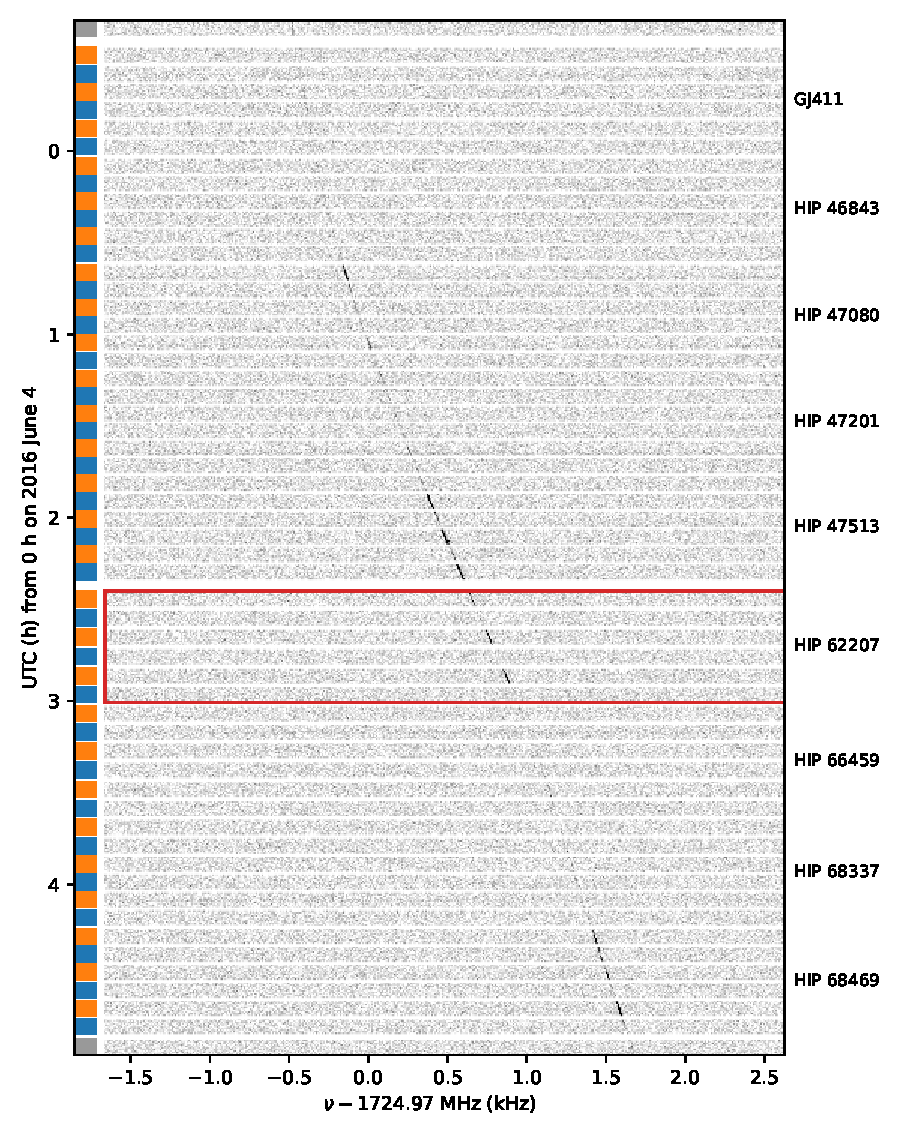
\includegraphics[width=0.82\textwidth]{mlc8_session.pdf}
\caption{Session AGBT16A\_999\_213 near MLc8: every scan's $16$ spectra at their times, in the $2.84$\,Hz channels,
each over a level from block medians of its median spectrum and scaled to unit noise, with the ON scans marked orange,
the OFF scans blue and the scans outside a cadence grey, and the cadence of HIP~62207 boxed. Each cadence is labelled
by its target.}
\label{fig:mlc8}
\end{figure}

MLc1 is the one signal its session does not settle. It lies on its line in its three ON scans, at $3.80$, $7.10$ and
$3.43$ against parallel tracks at $0.14$ to $0.26$ with a scatter of $0.69$ to $0.88$, $4$ to $9\sigma$ each; in its
first OFF scan at $2.16$ against $0.27\pm0.70$, $2.7\sigma$, and not in the other two; and in no scan pointed at another star of its
session, which holds $27$ scans from 15:17 to 17:59\,UTC on 2016 June 2. Its strongest tracks in the first two ON scans
drift at $-1.51$ and $-0.85$\,\hzs. A transmitter at rest at HIP~13402 would drift at $-0.08$\,\hzs, so one at the
star would need a line-of-sight acceleration of its own of $0.23$\,\mss, changing by $0.17$\,\mss\ in the $12$ minutes
between those scans. At $1188.54$\,MHz it lies in the $960$--$1215$\,MHz band of aeronautical radionavigation, used by
DME and TACAN beacons and by the GPS L5, Galileo E5 and BeiDou B2 signals of $1164$--$1215$\,MHz.

% =============================================================================
\section{Related work}\label{sec:related}
% =============================================================================

Sheikh et al.~\cite{Sheikh2021} examined blc1, a signal from the direction of Proxima Centauri, by finding look-alikes
of it at related frequencies in observations of other targets, and set out the verification framework that a trace
through the session follows. Pardo et al.~\cite{Pardo2025} passed Ma et al.'s eight through the filters of an anomaly
search. We find no earlier analysis of the eight beyond their cadences.

% =============================================================================
\section{Conclusion}\label{sec:conclusion}
% =============================================================================

A cadence holds six scans of a session that holds tens. Traced through their sessions in the $2.84$\,Hz product, seven
of Ma et al.'s eight signals of interest are transmitters on the ground that the ON--OFF test passed because the
telescope received them more weakly in three OFF pointings; the trace reads one coarse channel of each scan and
settles them without re-observation. MLc1 remains, in the band of aeronautical radionavigation with a drift that
changes by $0.66$\,\hzs\ between scans $12$ minutes apart; the Doppler rates at the GBT of the navigation satellites
above it on 2016 June 2 between 16:34 and 16:58\,UTC would decide whether one of them carried it.

\section*{Acknowledgements}

This work uses data from Breakthrough Listen, funded by the Breakthrough Prize Foundation, taken with the Green Bank
Telescope; the Green Bank Observatory is a facility of the National Science Foundation operated under cooperative
agreement by Associated Universities, Inc. It uses the SIMBAD database, operated at CDS, Strasbourg, and Astropy.

\begin{thebibliography}{99}\small\raggedright
\setlength{\itemsep}{1pt}

\bibitem{Ma2023}
P.~X. Ma, C.~Ng, L.~Rizk, et al., A deep-learning search for technosignatures from 820 nearby stars, \emph{Nat.
Astron.} \textbf{7}, 492 (2023).

\bibitem{Pardo2025}
S.~Pardo, D.~Poznanski, S.~Croft, A.~P.~V. Siemion and M.~Lebofsky, Using anomaly detection to search for
technosignatures in Breakthrough Listen observations, \emph{Astron. J.} \textbf{170}, 12 (2025).

\bibitem{Isaacson2017}
H.~Isaacson, A.~P.~V. Siemion, G.~W. Marcy, et al., The Breakthrough Listen search for intelligent life: target
selection of nearby stars and galaxies, \emph{Publ. Astron. Soc. Pac.} \textbf{129}, 054501 (2017).

\bibitem{Enriquez2017}
J.~E. Enriquez, A.~Siemion, G.~Foster, et al., The Breakthrough Listen search for intelligent life: 1.1--1.9\,GHz
observations of 692 nearby stars, \emph{Astrophys. J.} \textbf{849}, 104 (2017).

\bibitem{MacMahon2018}
D.~H.~E. MacMahon, D.~C. Price, M.~Lebofsky, et al., The Breakthrough Listen search for intelligent life: a wideband
data recorder system for the Robert C. Byrd Green Bank Telescope, \emph{Publ. Astron. Soc. Pac.} \textbf{130}, 044502
(2018).

\bibitem{Lebofsky2019}
M.~Lebofsky, S.~Croft, A.~P.~V. Siemion, et al., The Breakthrough Listen search for intelligent life: public data,
formats, reduction, and archiving, \emph{Publ. Astron. Soc. Pac.} \textbf{131}, 124505 (2019).

\bibitem{Sheikh2021}
S.~Z. Sheikh, S.~Smith, D.~C. Price, et al., Analysis of the Breakthrough Listen signal of interest blc1 with a
technosignature verification framework, \emph{Nat. Astron.} \textbf{5}, 1153 (2021).

\end{thebibliography}

\end{document}
